\documentclass[11pt, oneside]{article}   	% use "amsart" instead of "article" for AMSLaTeX format
\usepackage{geometry}                		% See geometry.pdf to learn the layout options. There are lots.
\geometry{letterpaper}                   		% ... or a4paper or a5paper or ... 
%\geometry{landscape}                		% Activate for for rotated page geometry
%\usepackage[parfill]{parskip}    		% Activate to begin paragraphs with an empty line rather than an indent
\usepackage{graphicx}				% Use pdf, png, jpg, or eps� with pdflatex; use eps in DVI mode
								% TeX will automatically convert eps --> pdf in pdflatex		
\usepackage{amssymb}
\usepackage{amsmath}
\usepackage{parskip}
\usepackage{color}
\usepackage{hyperref}

\title{The limit of x/sin x}
%\author{The Author}
%\section{}
%\subsection*{}
\date{}							% Activate to display a given date or no date

\graphicspath{{/Users/telliott_admin/Dropbox/Tex/png/}}
% \begin{center} 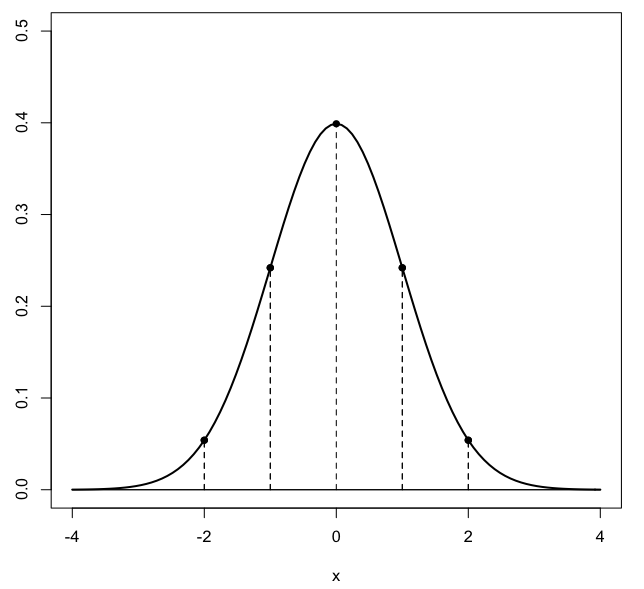
\includegraphics [scale=0.4] {gauss3.png} \end{center}
\begin{document}
\maketitle
\Large
The fundamental result of calculus with respect to trigonometric functions depends on
\[ \lim_{x \rightarrow 0} \ \frac{x}{\sin x} \]
The ratio of the angle to its sine as the angle gets very small.  Here is a simple proof that the ratio is equal to $1$.
\begin{center} 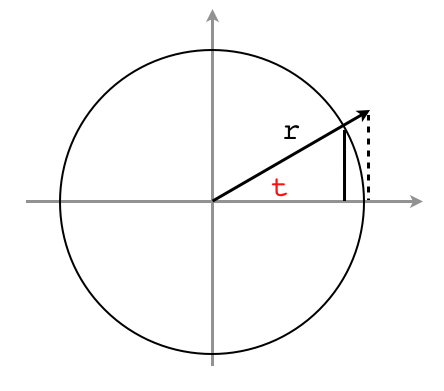
\includegraphics [scale=0.4] {lim_x_over_sinx.png} \end{center}
Consider the triangle that lies entirely inside the circle.  Its base is $r \cos t$ and its height is $r \sin t$, so its area is
\[ A = \frac{1}{2} \cdot r \cos t \cdot r \sin t = \frac{1}{2} r^2 \sin t \cos t \]
Consider next the segment of the circle with angle $t$.  Its area is that fraction of $2 \pi$ times the total area
\[ A = \frac{t}{2 \pi} \pi r^2 = \frac{1}{2} r^2 t \]
Finally, consider the dotted line.  By similar triangles its length is in the same ratio to $r$ (which is the base of that triangle), as sine is to cosine of the angle.  That is, its length is $r \tan t$ and so the area of the triangle is
\[ A = \frac{1}{2} \cdot r \cdot r \tan t =  \frac{1}{2} r^2 \ \frac{\sin t}{\cos t} \]
Since these areas get progressively larger
\[ \frac{1}{2} r^2 \sin t \cos t < \frac{1}{2} r^2 t < \frac{1}{2} r^2 \ \frac{\sin t}{\cos t} \]
Now divide by $(1/2)r^2 \sin t$
\[ \cos t < \frac{t}{\sin t} < \frac{1}{\cos t} \]
Now, as $t \rightarrow 0$, both $\cos t$ and $1/\cos t$ also go to $1$.  Therefore the ratio gets squeezed, and it goes to $1$ as well.  Thus
\[ \lim_{x \rightarrow 0} \ \frac{x}{\sin x} = 1 \]

There is another limit that also comes up in the basic derivations, but it turns out to be related to this one.  That limit is:

\end{document}  